\documentclass[12pt]{article}
\usepackage[utf8]{inputenc}
\usepackage{listingsutf8}
\usepackage{color} 
\usepackage{tikz-uml}
\usepackage{graphicx}
\usepackage{geometry}
\geometry{a4paper,left=2.5cm, right = 2cm , top= 3cm, bottom = 3cm}
\setlength{\parindent}{0cm}
\definecolor{codegreen}{rgb}{0,0.6,0}
\definecolor{codegray}{rgb}{0.5,0.5,0.5}
\definecolor{codepurple}{rgb}{0.58,0,0.82}
\definecolor{backcolour}{rgb}{0.9,0.90,0.84} 
\lstdefinestyle{mystyle}{
    backgroundcolor=\color{white},   
    commentstyle=\color{codegreen},
    keywordstyle=\color{blue},
    numberstyle=\tiny\color{codegray},
    stringstyle=\color{codepurple},
    basicstyle=\footnotesize,
    breakatwhitespace=false,         
    breaklines=true,                 
    captionpos=b,                    
    keepspaces=true,                 
    %este comando sirve para habilitar la presencia de la linea de numeros
    numbers=left,                        
    numbersep=5pt,                  
    showspaces=false,                
    showstringspaces=false,
    showtabs=false,                  
    tabsize=2
}
 
\lstset{style=mystyle,
inputencoding=latin1}
\usepackage{fancyhdr}
\pagestyle{fancy}
\fancyhead{
\lhead{UMSA}
\chead{lab-121}
\rhead{Informática}
}											% No page header
\fancyfoot[L]{Marco Antonio Vino}											% Empty 
\fancyfoot[C]{}											% Empty
\fancyfoot[R]{\thepage}									% Pagenumbering
\renewcommand{\headrulewidth}{1pt}			% Remove header underlines
\renewcommand{\footrulewidth}{0.5pt}				% Remove footer underlines
\setlength{\headheight}{5pt}




%%% Maketitle metadata
\newcommand{\horrule}[1]{\rule{\linewidth}{#1}} 	% Horizontal rule

\title{
		%\vspace{-1in} 	
		\usefont{OT1}{bch}{b}{n}
		\normalfont \normalsize \textsc{Universidad Mayor de San Andres \\
        Facultad de Ciencias Puras y Naturales\\
        Carrera de Informática \\
        lab-121\\
        Lic. Cecilia E. Tarquino P.} \\ [25pt]
		\horrule{0.5pt} \\[0.2cm]
		\huge PROYECTO: Seguimiento de prestamos de material  \\
       \horrule{2pt} \\[0.1cm]
}

\author{
		\normalfont 								\normalsize
        Marco Antonio Vino Chipana	 \\
        CI 9111299 L.P.\\
        29 de noviembre de 2018\\[-3pt]		\normalsize        
}
\date{}
\begin{document}

%\begin{center}
%\maketitle
 
%\section*{Práctica \#1 \\ Comandos para manejo de directorios, archivos y permisos}
%\end{center}
\maketitle 
\thispagestyle{empty}

\newpage
\section{Introducción}

Cuando se tiene que llevar el registro de los prestamos que se realizan en alguna institución, nos encontramos con el problema de que este dbe ser oportuno, rápido y eficiente.  En este caso de estudio lo que vamos a realizar es el modelado y programación de un sistema de control de prestamos.  
Este sistema se desarollará utilizando en entorno gráfico que nos facilitan las aplicaciones de Windows Forms. Se utilizará el lenguaje de programación C\#, dentro del entorno de desarrollo SharpDevelop en su versión 5.1.  \\

De la misa forma se utilizan los conceptos de la programación orientada a objetos, tales como al herencia, la sobrecarga, las clases y objetos, la agregación , la composición y la persistencia de archivos.  

\section{Análisis del ambiente y el problema}
\subsection{Estado del arte}
Como primer recurso se utilizará un inventario, el cual es una relación detallada, ordenada y valorada de los elementos que componen el patrimonio de una empresa o persona en un momento determinado. 
\begin{center}

\includegraphics[scale=0.4]{IMG/inventario.jpg} \\ 

\end{center}

El segundo elemento serán los usuarios, en informática un usuario es una persona que utiliza una aplicación o sistema a través del uso de una computadora, la cual para su utilización requiere cierto nivel de experticia.  
\begin{center}

\includegraphics[scale=0.4]{IMG/usuarios.png} \\ 

\end{center}

Cada uno de los recursos que se podrán utilizar serán considerados ítems,  Consideraremos como un ítem a cada uno de los recursos  físicamente separables que puedan ser prestados individualmente, como ser, un tubo de ensayo, un mortero, etc.  
\begin{center}

\includegraphics[scale=0.4]{IMG/recursos.jpg} \\ 

\end{center}



\subsection{Problemática}
Debemos llevar un registro del historial de los préstamos a los usuarios para poder saber su confiabilidad y si es que tienen o no sanciones por incumplimiento de reglas \\
Alertar al administrador cuando los materiales no han sido devueltos en los plazos establecidos para poder hacer in seguimiento. \\
Saber en tiempo real la disponibilidad de recursos para poder solicitarlos en préstamo.  \\
Tener un estimado de cuando debería estar disponible el recurso que necesitamos para poder hacer una planificación. \\
Averiguar la rotación de los elementos para ver la demanda de recursos  y utilizar esta información para futuras adquisiciones, generando preferencias por aquellos elementos que más se hayan encontrado agotados en varias situaciones. 

\section{Objetivos}
\subsection{Objetivo general}
Realizar seguimiento al movimiento de los recursos susceptibles a préstamo dentro de una institución.  
\subsection{Objetivos específicos}
\begin{itemize}
\item Registrar todos los préstamos de material
\item Identificar a todos los usuarios que pueden prestarse material
\item Registrar las devoluciones del material
\item Mostrar en tiempo real la disponibilidad de materiales
\item Consultar quien tiene prestado un material con identificacion x.
\item Consultar que recursos debe el estudiante X.  

\end{itemize}
\newpage
\section{Diagrama de clases}
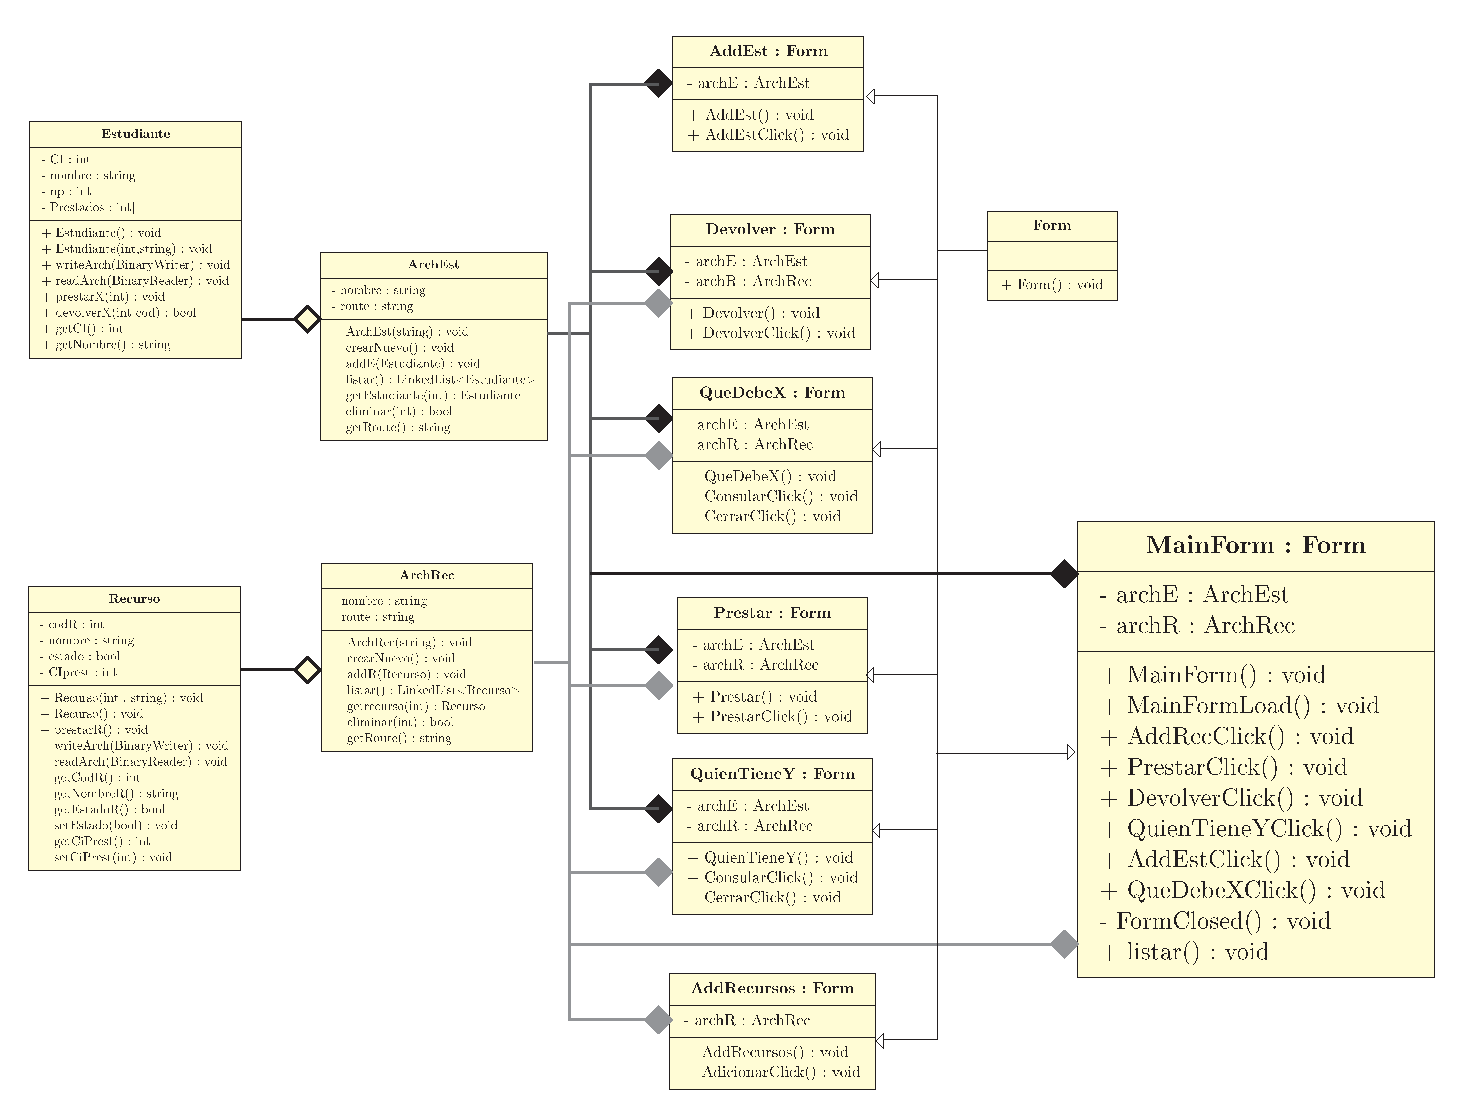
\includegraphics[scale=0.89, angle = -90]{UML/Diagrama.pdf}

\newpage
\section{Descripción de las clases}
\subsection{Clases más importantes del desarrollo}
En esta sección se describirán las clases propias del desarrollo más allá del entorno gráfico que fueron utilizadas durante el desarrollo para cumplir nuestros objetivos.
\subsubsection{Estudiante}
\begin{center}
\begin{tikzpicture}
\umlclass{Estudiante}
{ - CI : int \\
-  nombre : string \\
- np : int \\
- Prestados: int[]\\
}
{
+ Estudiante() : void\\
+ Estudiante(int,string) : void\\
+ writeArch(BinaryWriter) : void\\
+ readArch(BinaryReader) : void\\
+ prestarX(int) : void\\
+ devolverX(int cod) : bool\\
+ getCI() : int\\
+ getNombre() : string\\
}
\end{tikzpicture}

\end{center}
Esta clase guarda la información de cada estudiante, con su \textit{nombre} , su \textit{C.I.}  además de todos los recursos que se ha prestado.  \\ 
El método \textbf{prestarX(int)} agrega un recurso a la lista de presados del estudiante.  El método \textbf{devolverX(int)} elimina de la lista de recursos prestados al estudiante, aquel que tenga el código que se pasa como argumento, retorna verdadero si se pudo realizar la devolución y falso si hubo algún fallo.  

\subsubsection{Archivo Estudiante}
\begin{center}
\begin{tikzpicture}
\umlclass{ArchEst}
{ - nombre : string\\
- route : string\\
}
{ + ArchEst(string) : void\\
+ crearNuevo() : void\\
+ addE(Estudiante) : void\\
+ listar() : LinkedList<Estudiante>\\
+ getEstudiante(int): Estudiante\\
+ eliminar(int) : bool\\
+ getRoute() : string}
\end{tikzpicture}
\end{center}

Es la clase que realiza el manejo del archivo donde se guardan todos los estudiantes.  Como atributos tiene el \textit{nombre }del archivo, además de su \textit{ruta}.  El método \textbf{addE(Estudiante)}, agrega al estudiante que pasamos como argumento al final del archivo.  La función \textbf{listar()} nos permite extraer una lista que contiene a todos los estudiantes guardados en el archivo. la función \textbf{getEstudiente(int)} extrae al estudiante cuyo carnet se pasó como argumento.  El método \textbf{eliminar(int)} borra del archivo al estudiante cuyo carnet se haya ingresado como argumento. 

\subsubsection{Recurso}
\begin{center}
\begin{tikzpicture}
\umlclass{Recurso}
{- codR : int\\
- nombre : string\\
- estado : bool\\
- CIprest : int}
{
+ Recurso(int , string) : void\\
+ Recurso() : void\\
+ prestarR() : void\\
+ writeArch(BinaryWriter) : void\\
+ readArch(BinaryReader) : void\\
+ getCodR() : int\\
+ getNombreR() : string\\
+ getEstadoR() : bool\\
+ setEstado(bool) : void\\
+ getCiPrest() : int \\
+ setCiPrest(int) : void
}
\end{tikzpicture}
\end{center}

La clase recurso se utiliza para guardar la información de un elemento suceptible a prestamo dentro de nuestro sistema, tiene como atributos un identificador único denotado por \textit{codR}, además de un \textit{nombre}, un \textit{estado} (que es verdadero si está en préstamo y falso si no), además de un \textit{CiPrest}, para saber a quien se le prestó el recurso.   \\ 
El método \textbf{prestar()} cambia el estado de un recurso a verdadero, el método \textbf{setCiPrest(int)} pone como persona a quien se prestó el recurso, aquella que tenga el carnet ingresado.  De la misma forma \textbf{setEstado(bool)} nos sirve para cambiar el estado del recurso.  

\subsubsection{Archivo Recurso}
\begin{center}
\begin{tikzpicture}
\umlclass{ArchRec}
{ - nombre : string\\
- route : string\\
}
{ + ArchRec(string) : void\\
+ crearNuevo() : void\\
+ addR(Recurso) : void\\
+ listar() : LinkedList<Recurso>\\
+ getrecurso(int): Recurso\\
+ eliminar(int) : bool\\
+ getRoute() : string}

\end{tikzpicture}\\
\end{center}

Es la clase que realiza el manejo del archivo donde se guardan todos los Recursos.  Como atributos tiene el \textit{nombre }del archivo, además de su \textit{ruta}.  El método \textbf{addR(Recurso)}, agrega un nuevo Recurso, el que pasamos como argumento al final del archivo, por defecto setea el estado como disponible.  La función \textbf{listar()} nos permite extraer una lista que contiene a todos los recursos guardados en el archivo. la función \textbf{getrecurso(int)} extrae al recurso con el código que se pasó como argumento.  El método \textbf{eliminar(int)} borra del archivo al recurso cuyo código se haya ingresado como argumento. 


\subsection{Clases de los formularios del entorno gráfico}
Se describirán como funcionan los diferentes formularios desarrollados dentro del entorno gráfico del proyecto.  


\subsection{Formulario principal}
\begin{tikzpicture}
\umlclass{MainForm : Form}
{ - archE : ArchEst\\
- archR : ArchRec\\
}{ + MainForm() : void \\
+ MainFormLoad() : void \\
+ AddRecClick() : void\\
+ PrestarClick() : void\\
+ DevolverClick() : void\\
+ QuienTieneYClick() : void\\
+ AddEstClick() : void\\
+ QueDebeXClick() : void\\
- FormClosed() : void\\
+ listar() : void
}

\pgftext[x=250, y=0]{\includegraphics[width=300pt]{IMG/MainForm.png}} ;
\end{tikzpicture}

El formulario principal es el que se abre al inicio del sistema,  el mismo tiene como atributos a los archivos tanto de \textit{estudiantes} como de \textit{recursos}.  Su función principal es mostrar el estado de las diferentes listas, y esto se lleva a cabo del método \textbf{listar()}, cada uno de los botones tiene un método que abre otra ventana para la interacción,  por ejemplor \textbf{AddRecClick()} es un método que abré el formulario que nos permite agregar un nuevo recurso.  
De la misma forma \textbf{PrestarClick()} abre la ventana para registrar un prestamo.  El método \textbf{FormClosed()} nos sirve para actualizar la vista de elementos cada vez que se cierra una ventana de introducción de datos.  
Los métodos \textbf{QuienTieneY()} y \textbf{QueDebeX()} abren ventanas de consulta para cada una de sus tareas.

  
\subsubsection{Agregar Recurso}

\begin{tikzpicture}
\umlclass{AddRecursos : Form}
{ - archR : ArchRec\\
}{ + AddRecursos() : void \\
+ AdicionarClick() : void\\
}

\pgftext[x=250, y=0]{\includegraphics[width=200pt]{IMG/AddRecurso.png}} ;
\end{tikzpicture}

Esta ventana nos permite agregar un recurso más a la lista de recursos guardaas en el archivo \textbf{ArchRec}.  Esta funcionalidad es llevada a cabo por el método \textbf{AdicionarClick()}, que se ejecuta cuando le damos click al boton adicionar.  Para poder ser llevado a cabo realiza las comprobaciones necesarias de que el código sea un número válido.  

\subsubsection{Prestar recurso}

\begin{tikzpicture}
\umlclass{Prestar : Form}
{  - archE : ArchEst\\
- archR : ArchRec\\
}{ + Prestar() : void \\
+ PrestarClick() : void\\
}

\pgftext[x=250, y=0]{\includegraphics[width=200pt]{IMG/Prestar.png}} ;
\end{tikzpicture}

Tiene como atributos tanto los archivos de estudiante como los de recursos para poder registrar los cambios.  
Esta ventana nos sirve para registrar los préstamos que se realizan en el sistema.  Tiene 3 elementos a ser llenados, la fecha, el ci de la persona a la que se le prestará y el cod del recurso que se presta.  Dentro del método \textbf{PrestarClick()} se realizan las comprobaciones para que los datos ingresados sean válidos.  Se cambia el estado del recurso ingresado, además que se le asigna al atributo CiPrest el carnet de la persona que se presto el recurso.  Al mismo tiempo, Al estudiante con el ci ingresado se le agrega el recurso a articulos prestados siempre y cuando este disponible. 


\subsubsection{Devolver recurso}
\begin{tikzpicture}
\umlclass{Devolver : Form}
{  - archE : ArchEst\\
- archR : ArchRec\\
}{ + Devolver() : void \\
+ DevolverClick() : void\\
}


\pgftext[x=250, y=0]{\includegraphics[width=200pt]{IMG/Devolver.png}} ;
\end{tikzpicture}

Tiene como atributos tanto los archivos de estudiante como los de recursos para poder registrar los cambios.  
El método \textbf{DevolverClick()}, verifica que los datos ingresados sean válidos y cambia el estado del recurso con el cod ingresado, además que eliminar de las lista de prestados del estudiante con el CI ingresado, el recurso que esta devolviendo.  


\subsubsection{¿Quién tiene el recurso Y?}
\begin{tikzpicture}
\umlclass{QuienTieneY : Form}
{  - archE : ArchEst\\
- archR : ArchRec\\
}{ + QuienTieneY() : void \\
+ ConsularClick() : void\\
+ CerrarClick() : void
}

\pgftext[x=250, y=0]{\includegraphics[width=200pt]{IMG/QuienTieneY.png}} ;
\end{tikzpicture}

Tiene como atributos tanto los archivos de estudiante como los de recursos para consultar los valores.  
El método \textbf{ConsultarClick()} Busca si el recurso con el código ingresado ha sido prestado, y si ha sido prestado, y si está prestado extrae el CIPrest, y busca en el \textit{ArchEst} los datos del estudiante que tiene el recurso consultado.  \\
El método \textbf{CerrarClick()}, cierra el formulario actual y envía la señal de actualizar al formulario principal.  

\subsubsection{Agregar Estudiante}

\begin{tikzpicture}
\umlclass{AddEst : Form}
{  - archE : ArchEst\\
}{ + AddEst() : void \\
+ AddEstClick() : void\\
}
\pgftext[x=250, y=0]{\includegraphics[width=200pt]{IMG/AddEstudiante.png}} ;
\end{tikzpicture}

Esta ventana nos permite agregar un estudiante más a la lista de estudiantes guardos en el archivo \textbf{ArchEst}.  Esta funcionalidad es llevada a cabo por el método \textbf{AdicionarClick()}, que se ejecuta cuando le damos click al boton adicionar.  Para poder ser llevado a cabo realiza las comprobaciones necesarias de que el CI sea un número válido.  

\subsubsection{¿Qué debe el estudiante X?}

\begin{tikzpicture}
\umlclass{QueDebeX : Form}
{  - archE : ArchEst\\
- archR : ArchRec\\
}{ + QueDebeX() : void \\
+ ConsularClick() : void\\
+ CerrarClick() : void
}
\pgftext[x=250, y=0]{\includegraphics[width=200pt]{IMG/QueDebeX.png}} ;
\end{tikzpicture}
Tiene como atributos tanto los archivos de estudiante como los de recursos para consultar los valores.  
En método \textbf{ConsultarClick()}, busca el valor de CI en el \textit{archE}, y si lo encuentra pasa a buscar dentro del \textit{archR} todos aquellos recursos que se hayan prestado con ese CI y los va mostrando en el data grid view.  \\
El método \textbf{CerrarClick()}, cierra el formulario actual y envía la señal de actualizar al formulario principal.  
\newpage
\section{Herramientas y librerias utilizadas}
\subsection{C\#}
C\# es un lenguaje de programación orientado a objetos desarrollado y estandarizado por Microsoft como parte de su plataforma .NET. 

Su sintaxis básica deriva de C/C++ y utiliza el modelo de objetos de la plataforma .NET, similar al de Java, aunque incluye mejoras derivadas de otros lenguajes.

El nombre C Sharp fue inspirado por el signo '\#' que se compone de cuatro signos '+' pegados.  

las Librerias utilizadas en el desarrollo del proyecto se detallan a continuación.  

\begin{itemize}
\item \textbf{System} contiene clases fundamentales y clases básicas que definen tipos de datos de valor y referencia comúnmente utilizados, eventos y controladores de eventos, interfaces, atributos y excepciones de procesamiento.
\item \textbf{System.Collections.Generic} contiene interfaces y clases que definen colecciones genéricas, que permiten a los usuarios crear colecciones tipificadas con fuerza que proporcionan una seguridad y rendimiento de tipo mejor que las colecciones tipográficas no genéricas.
\item \textbf{System.Windows.Forms} contiene clases para crear aplicaciones basadas en Windows que aprovechan al máximo las características de la interfaz de usuario ricas disponibles en el sistema operativo Microsoft Windows.
\end{itemize}
\subsection{SharpDevelop 5.1}

SharpDevelop es un entorno de desarrollo integrado libre desarrollado por \textit{ICSharpCode Team}, con su última version 5.1 lanzada el 14 de abril de 2016. 

Para el completado automático de código, la aplicación incorpora sus propios analizadores sintácticos.  Además que integra la funcionalidad de trabajar en el entorno de Windows Forms. 

\subsection{\LaTeX}

\LaTeX es un sistema de composición de textos de código abierto, orientado a la creación de documentos escritos que presenten una alta calidad tipográfica. Por sus características y posibilidades, es usado de forma especialmente intensa en la generación de artículos y libros científicos que incluyen, entre otros elementos, expresiones matemáticas. 

Específicamente las librrerias que se utilizaron en este proyecto son: 

\begin{itemize}
\item  \textbf{listingsutf8} nos permite mostrar el código fuente en un documento, directamente desde el archivo que contiene el código fuente.  
\item \textbf{tikz-uml} que nos permite desarrollar los diagramas UML de manera sencilla y directa.
\end{itemize}

\newpage
\section{Código fuente}
\subsection{Clases más importantes}
\textbf{Clase Estudiante: }
\lstinputlisting[language = Java]{../Prestamos/Codigo/Estudiante.cs}
\textbf{Clase Archivo Estudiante: }
\lstinputlisting[language = Java]{../Prestamos/Codigo/ArchEst.cs}
\textbf{Clase Recurso: }
\lstinputlisting[language = Java]{../Prestamos/Codigo/Recurso.cs}
\textbf{Clase Archivo Recurso: }
\lstinputlisting[language = Java]{../Prestamos/Codigo/ArchRec.cs}
\subsection{Clases del entorno gráfico}
\textbf{Clase del formulario principa:l}
\lstinputlisting[language = Java]{../Prestamos/MainForm.cs}
\textbf{Clase del formulario agregar estudiante: }
\lstinputlisting[language = Java]{../Prestamos/AddEst.cs}
\textbf{Clase del formulario agregar recurso: }
\lstinputlisting[language = Java]{../Prestamos/AddInst.cs}
\textbf{Clase formulario registro devolución recurso}
\lstinputlisting[language = Java]{../Prestamos/Devolver.cs}
\textbf{Clase formulario registro préstamo de recurso}
\lstinputlisting[language = Java]{../Prestamos/Prestar.cs}
\textbf{Clase formulario consulta que debe el estudiante X}
\lstinputlisting[language = Java]{../Prestamos/QueDebeX.cs}
\textbf{Clase formulario consulta quien tiene el recurso Y}
\lstinputlisting[language = Java]{../Prestamos/QuienTieneY.cs}
\textbf{Clase que inicializa el formulario principal}
\lstinputlisting[language = Java]{../Prestamos/Program.cs}
\newpage
\section{Ejecución del programa}
\begin{itemize}

\item[\textbf{1)}] Agregar un recurso a la central de préstamos.
\begin{center}
\begin{tikzpicture}
\pgftext[x=0, y=0]{\includegraphics[scale=0.5]{IMG/Work/Estado1.png}} 
\pgftext[x=-100, y= -170]{\includegraphics[scale=0.5]{IMG/Work/Estado2.png}}
\end{tikzpicture}
\end{center}
Inicialmente no tenia el recurso \textbf{microscopio }con el \textbf{código 8}, pero despues e la ejecución se lo tiene registrado.  La función que permite esta adición es \textbf{Button1Click()} del Formulario \textit{addRecurso}. 
\lstinputlisting[language = Java, firstline= 19, lastline = 35]{../Prestamos/AddInst.cs}




\newpage
\item[\textbf{2)}] Agregar un estudiante a la central de préstamos.
\begin{center}
\begin{tikzpicture}
\pgftext[x=0, y=0]{\includegraphics[scale=0.5]{IMG/Work/Estado3.png}} 
\pgftext[x=-100, y= -170]{\includegraphics[scale=0.5]{IMG/Work/Estado4.png}}
\end{tikzpicture}
\end{center}
Inicialmente no tenia el estudiante \textbf{Roberto Gonzales }con el \textbf{CI 4568521}, pero despues e la ejecución se lo tiene registrado.  La función que permite esta adición es \textbf{Button1Click()} del Formulario \textit{addEstudiante}. 
\lstinputlisting[language = Java, firstline= 15, lastline = 30]{../Prestamos/AddEst.cs}



\newpage
\item[\textbf{3)}] Prestar un recurso disponible a un estudiante.
\begin{center}
\begin{tikzpicture}
\pgftext[x=0, y=0]{\includegraphics[scale=0.5]{IMG/Work/Estado5.png}} 
\pgftext[x=-100, y= -170]{\includegraphics[scale=0.5]{IMG/Work/Estado6.png}}
\end{tikzpicture}
\end{center}
Inicialmente el recurso  \textit{guitarra honner} con \textit{código 123}, estaba disponible. Pero se lo prestaron a la persona con CI 132465789.  Con lo que en la nueva vista pasa a la lista de prestados y desaparece de los disponibles.  El método que permite esto es el \textbf{Button1Click()} dentro del formulario \textit{Prestar}. 
\lstinputlisting[language = Java, firstline= 16, lastline = 43]{../Prestamos/Prestar.cs}

\item[\textbf{4)}] registrar la devolución de un recurso prestado a un estudiante.
\begin{center}
\begin{tikzpicture}
\pgftext[x=0, y=0]{\includegraphics[scale=0.5]{IMG/Work/Estado7.png}} 
\pgftext[x=-100, y= -170]{\includegraphics[scale=0.5]{IMG/Work/Estado8.png}}
\end{tikzpicture}
\end{center}
En las pantallas se muestra la devolución el recurso con \textit{código 123} del \textit{estudiante 132465789}, esto se lleva a cabo dentro del formulario \textit{Devolver} con el método \textbf{Button1Click()}.  
\lstinputlisting[language = Java, firstline= 18, lastline = 47]{../Prestamos/Devolver.cs}



\item[\textbf{5)}] Consultar ¿Qué estudiante tiene prestado el recurso Y?.

\begin{center}
\begin{tikzpicture}
\pgftext[x=0, y=-0]{\includegraphics[scale=0.5]{IMG/Work/Estado9.png}} 
\end{tikzpicture}
\end{center}
Al ingresar al boton ¿Quien tiene el recurso Y?, se despliega una nueva ventana que nos permite hacer la consulta en base al código del recurso.  En este caso se pregunto por el recurso con el \textit{código 654}, y nos muestra que lo tiene \textit{Marco Antonio Vino}, esto se realiza a través del método \textbf{ConsultarClick()} del formulario \textit{QuienTieneY}.  

\lstinputlisting[language = Java, firstline= 19, lastline = 43]{../Prestamos/QuienTieneY.cs}




\item[\textbf{6)}] Consultar los recursos que tiene prestado el estudiante X.

\begin{center}
\begin{tikzpicture} 
\pgftext[x=0, y=0]{\includegraphics[scale=0.5]{IMG/Work/Estado10.png}}
\end{tikzpicture}
\end{center}
Al ingresar al boton ¿Qué tiene el estudiante X?, se despliega una nueva ventana que nos permite hacer la consulta en base al \textit{CI} del estudiante.  En este caso se pregunto por el Estudiante con el \textit{CI 9111299}, y nos muestra Su nombre\textit{Marco Antonio Vino} además de una lista de los recursos que se le pretaron, esto se realiza a través del método \textbf{ConsultarClick()} del formulario \textit{QuéDebeX}.  

\lstinputlisting[language = Java, firstline= 15, lastline = 38]{../Prestamos/QueDebeX.cs}
\end{itemize}

\section{Conclusiones}
Podemos observar que el desarrollo de uns sistema requiere de una planificaición, diseño y estructuración estrictos para poder ser realizados.   Tambien nuestra aplicación puede cumplir con todos los requerimientos iniciales del enunciado del trabajo.  

Las funcionalidades del mismo pueden ser ampliadas con desarrollos posteriores.  
\nocite{*}

\newpage
\section{Bibliografía}
\bibliographystyle{acm}
\bibliography{biblio}

  





\end{document}
